%!TEX root = ../crimson_throne_book_main.tex
% 2015-09-12
With Heldrin and Korwick safe, two of the three children living with the party in the villa are now out of harm's way. Heldrin joins his friend in the Endrin Academy while the companions head over to the old city hall to rescue the third and last missing lamb: Mouse. Korvosa's former townhall is situated in the quieter part of the island, up on Garrison Hill, quite close to the Palace of the Arkona family. Apparently the nobleman's name still carries enough weight to keep the emperor's men at bay. The high tower of the abandoned building is impressive. The companions figure they will have to climb it to the top floor, with the stories in between forming the perfect set-up for traps. Proceeding with caution the party locates and dismantles three traps on the lower floors.\hyperref[fig:Korvosa-Old-City-Hall-559764706]{ Climbing the tower turns out to be safe } , at least until the companions reach a very high-ceilinged room in which the stairs wind up to the top floor. About halfway up the stairs acid rain starts pouring down on the heroes, burning their flesh. Balian scurries all the way up to shut off the sprinkling system. One wooden trap door separates the party from their destination, but Puk and Balian find powerful magic protecting the lid. Quint sacrifices himself and suffers the effects of a  {\itshape symbol of pain} to open the trap door, while his friends hide on the floor underneath to keep out of the harmful magical blast. Next they storm through the hole, with Balian and Puk leading the way. \\

\begin{figure}[h]
	\centering
	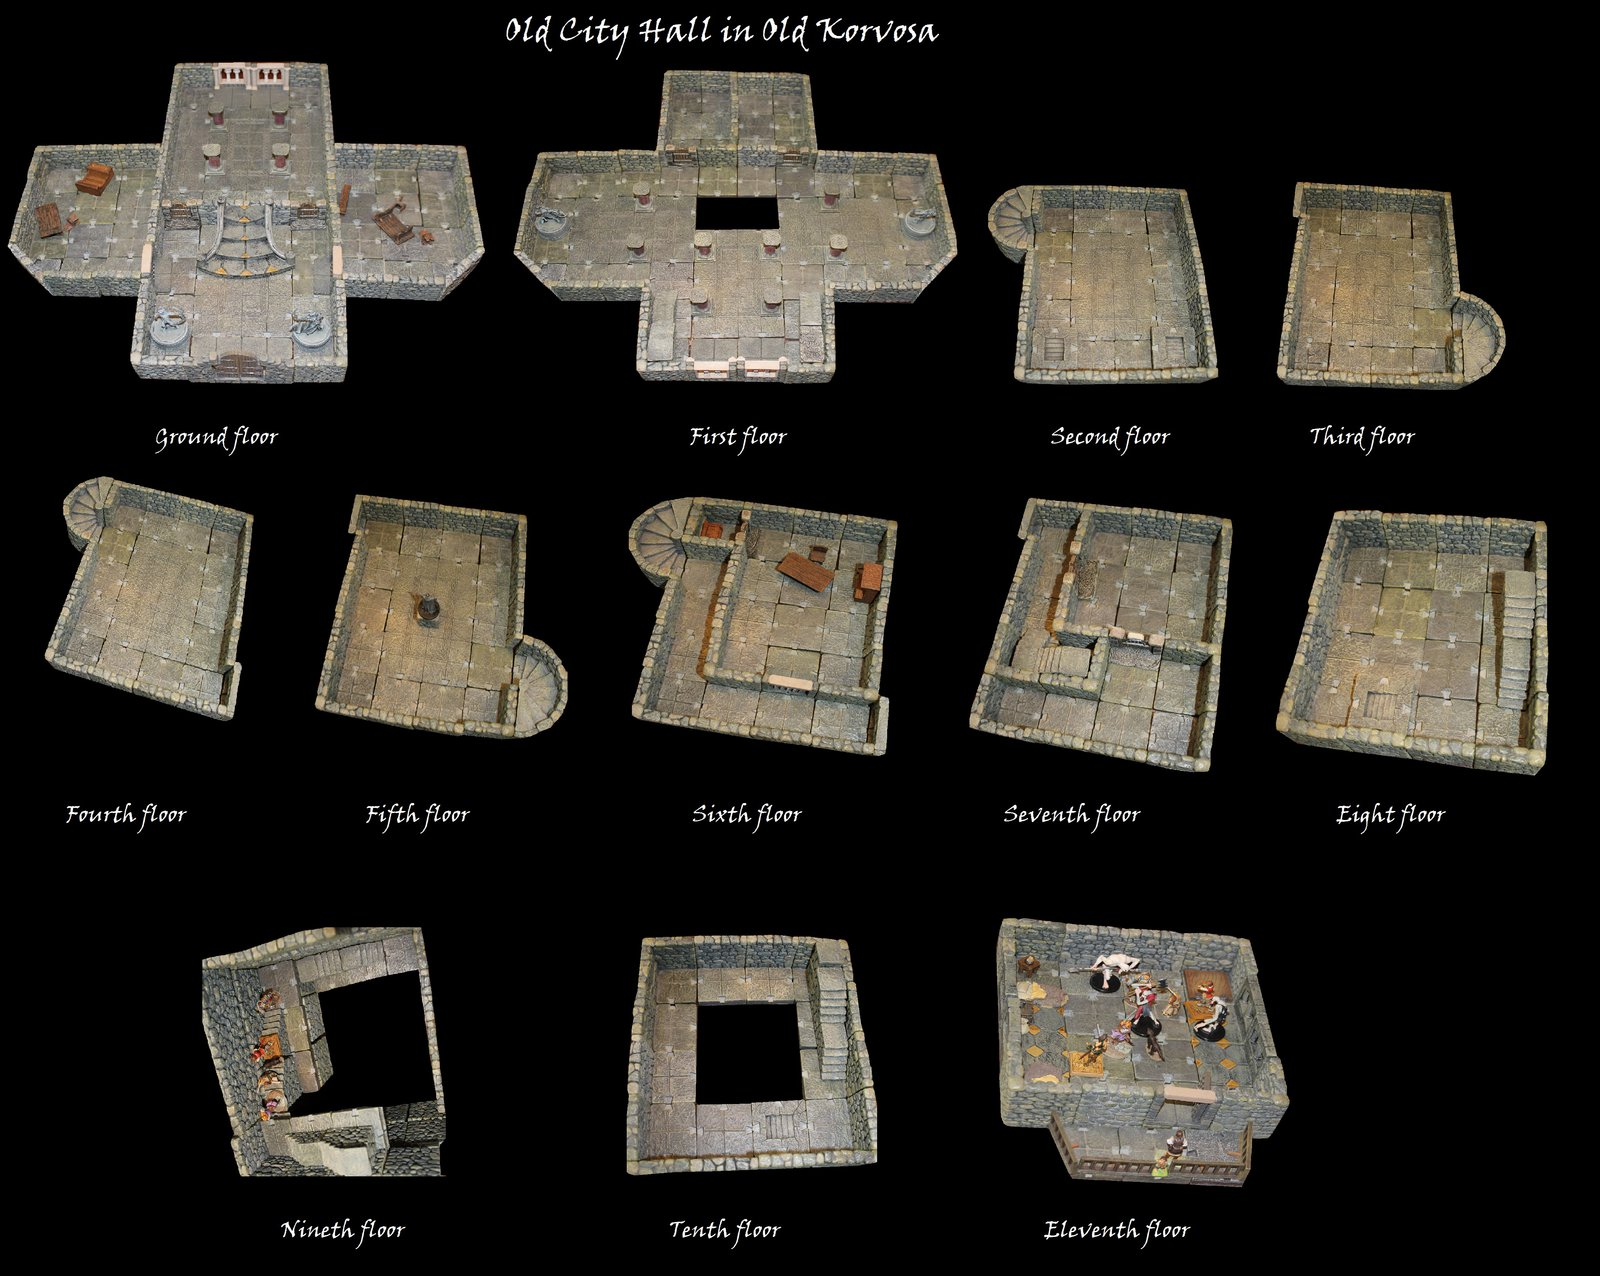
\includegraphics[width=0.39\textwidth]{images/Korvosa-Old-City-Hall-559764706.jpg}
	\caption{Korvosa Old City Hall}
	\label{fig:Korvosa-Old-City-Hall-559764706}
\end{figure}

The top room has windows on all sides, overlooking the region. There used to be a huge clock in here, but it was removed and melted down decades ago, when queen Domina needed funds to finance her ever growing hunger for fancy building projects. A balcony juts from the south side of the tower; the open door reveals Rolth standing in the wind. Tied up, on the other end of the railing, is Mouse. One nudge would suffice to push him down.\hyperref[fig:Final-showdown-with-Rolth-and-Alika-559765837]{ Barring the way to the door are three bearded devils and Alika. } Hate flickers in her eyes as her brother steps into view. "For the glory of Urgathoa! Time to settle the score!" she hisses as she removes a long leather glove from her right hand. Her limb is completely stripped of flesh, leaving nothing but bone, like an undead graft on living tissue. \\

\begin{figure}[h]
	\centering
	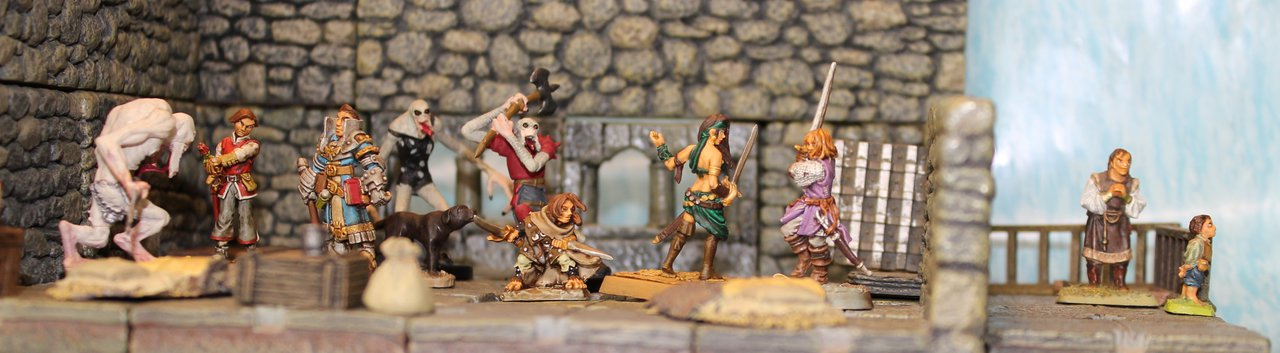
\includegraphics[width=0.39\textwidth]{images/Final-showdown-with-Rolth-and-Alika-559765837.jpg}
	\caption{Final showdown with Rolth and Alika}
	\label{fig:Final-showdown-with-Rolth-and-Alika-559765837}
\end{figure}

Sjo quickly gauges the situation and notices the schmuck smile on Rolth's ugly face, indicating that the necromancer feels in control with the little hostage at his mercy. The Shoanti summons his fiery wings and flies out, surprising the evil wizard and positioning himself between the foul man and his prey. Rolth looks most displeased and lifts off into the air himself ... he obviously prepared a {\itshape fly} spell. Still, he is frustrated, having hoped to threaten the party with the helpless boy and cast spells at them from a safe position. He calls into being a  {\itshape wall of force} that block the doorway and curses Sjo for ruining his plans once again. Sjo pulls Mouse over to the safe side of the railing and lifts off. The two flying men engage in an aerial dance, swirling around each other, trying to hurt one another with magic. Sjo easily withstands the burns of two scorching rays and scoffs at Rolth's attempt to  {\itshape fear} him, but he sees his own  {\itshape hold person} and  {\itshape dispel magic} fail as well. Meanwhile Puk and Spyder are keeping the bearded devils occupied. One of the creatures claws into the halfling and rends his flesh with his filthy beard, while the other two wield glaives and cut Balian and his pet dog from a ten feet distance. Alika immediately charges her brother and starts hacking away at him. The ranger returns the favor by showing no mercy when he wields his greatsword. Doubt still creeps through his veins as he misses his target more than he hits it. Quint pulls out the {\itshape wand of cure serious wounds} and reverts to healing again. He also launches a discouraging  {\itshape satire} in infernal, weakening the devils' attacks. Puk has already taken considerable damage, but strengthened by Quint's cure, he survives long enough to cut down a bearded devil. Next thing he knows is darkness, as the glaive of another devil drops him as well. Alika's skeletal claw hit several times, but deprived of an opportunity to sneak, the rogue does limited damage. When Balian's strokes hit, they are much more harmful. Even when the ranger realizes his sister is close to death, he does not hold back. He drives his blade through his sibling's chest, finishing her off once and for all. The foul necromancer corrupted her beyond saving, Balian sadly realizes. Death was the only release from this mortal existence that was left to her. And since she was Balian's responsibility, the cruel task fell on him. Still, the time to mourn will have to wait, for there are two dangerous devils left. Quint revives Puk and joins him in cornering one of the opponents, leaving the other one for Balian and Spyder. The heroes now have the upper hand and finish the job in a few rounds. Outside the flying struggle continues. Rolth blasts Sjo with a powerful {\itshape lightning bolt} , but the Shoanti casts some healing magic and flings himself at the wizard, grappling him. Rolth curses even more in frustration and barely succeeds at mumbling the words of  {\itshape dimension door} . From one second to the other he disappears. Sjo figures out that the wizard has to flee to a place close-by that he is familiar with, like somewhere else in the tower. The Shoanti flies down to the front door, quaffing more healing potions on the way. He enters the front hall again and stumbles upon his opponent in there. He jumps the necromancer once more and grabs him in a choking hold. This time Rolth fails his effort to cast magic and fizzles his get-away  {\itshape teleport} spell. Sjo is determined not to let go of his prey and clasps his arm tightly around the man's throat, sending fire through his hands again and again. He only stops when he has no more fire left. Rolth's charred and lifeless body tumbles to the ground. The companions recover some loot and find a special document in Rolth's possessions. After surviving the explosive runes on the parchment, Quint discovers it holds the precise wording of an infernal contract between Rolth and a devil named Chyvvom, promising the necromancer the services of infernal creatures up to five times in return for his immortal soul. The companions do not regret having had to fight their way through the servants from hell, as they now realize that Rolth will pay the price for these creatures' assistance with eternal torture in the afterlife. A fitting fate for one so foul!\\

